\documentclass{article}
\usepackage[utf8]{inputenc}
\usepackage[spanish]{babel}
\usepackage{listings}
\usepackage{graphicx}
\usepackage{cite}

\begin{document}

\begin{titlepage}
    \begin{center}
        \vspace*{1cm}
            
        \Huge
        \textbf{Informe Parcial 1}
            
        \vspace{0.5cm}
        \LARGE
        Informática II
            
        \vspace{1.5cm}
            
        \textbf{Daniel Perez\\Miguel Serna\\Jorge Montaña}
            
        \vfill
            
        \vspace{0.8cm}
            
        \Large
        Departamento de Ingeniería Electrónica y Telecomunicaciones\\
        Universidad de Antioquia\\
        Medellín\\
        Abril de 2021
            
    \end{center}
\end{titlepage}

\tableofcontents

\section{Análisis del problema}
El primer reto era evidente, debíamos conectar 64 luces LED a la mínima cantidad de pines posibles, claro esta, haciendo uso del dispositivo 74CH595 presentado en la clase, para si poder ampliar la cantidad de salidas digitales.\\

Terminado con eso, podríamos empezar a buscar métodos para encender ciertos LED y dejar los otros apagados y así poder formar figuras con la matriz 8x8, la opción mas lógica sería primero encender todos los LED y poner dicha solución en la función 'Verificación'. A partir de la solución usada en la función 'Imagen', la usaríamos en 'Publik' para que almacene los 3 caracteres deseados e imprima uno por uno.\\

Además de eso, debíamos hacer uso del serial para darle indicaciones al usuario y para que pudiese ingresar el numero, letra o carácter deseado y  aclarar las restricciones en el manual de usuario y de este modo no generar errores.


\section{Algoritmo Implementado} \label{contenido}
Véase en el repositorio de Github.

\begin{lstlisting}



\end{lstlisting}
\section{Problemas de desarrollo} \label{conclulsion}
El principal de los problemas que se nos presento fue sobre como íbamos a indicar los valores que los LED debían tener para formar cada letra, al final decidimos realizarlo de la forma mas obvia y lógica, simplemente dando los valores en binario a cada fila para formar dicho carácter, por ejemplo, una fila completamente encendida seria '255', lo que es el equivalente en decimal a '11111111' y con esa misma lógica podríamos  'dibujar' las matrices fila por fia de cada letra. \\


El hecho de que debíamos tener presente el arreglo de todas las letras, números y emojis, se convirtió en un problema para poder reconocer y validar todo lo que podía ingresar el usuario, además que la complejidad y lo extenso que se convirtió del algoritmo, el circuito y de que estuviéramos los 3 trabajando simultáneamente daban cavida a retrasos por la lentitud de la página y de que si uno de los miembros borraba o agregaba algo, los otros dos no podían ver el cambio sino unos 10 segundos después.\\

Se nos presentaros algunos errores de conexion de los LED, llegamdo al punto de que se formaban las figuras, pero al reves.\\


\section{Evolución del algoritmo} \label{conclulsion}
\subsection{Día 1}
Dia 1, 17 de abril.
Implementamos un circuito en base a las conexiones mostradas en la clase del sábado, junto a la matriz 8x8 de los LED\\


    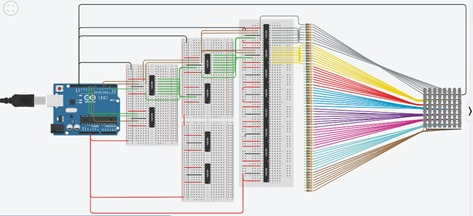
\includegraphics[width=12cm]{Dia 1.jpeg}



\subsection{Día 2}
Cambiamos significativamente el circuito, con el propósito principal de reducir la cantidad de pines usados lo máximo posible y logramos idear uno que solo hace uso de 3 pines, además de librarnos de posibles errores por tanta conexión.\\
Para el algoritmo inicializamos la estructura que íbamos a seguir, las salidas del SER, SRCLK,RCLK y tambíen el puerto serial. Iclusive, realizamos la primera funcion 'Verificacion' con éxito, dándole valores en binario como habíamos acordado antes.\\

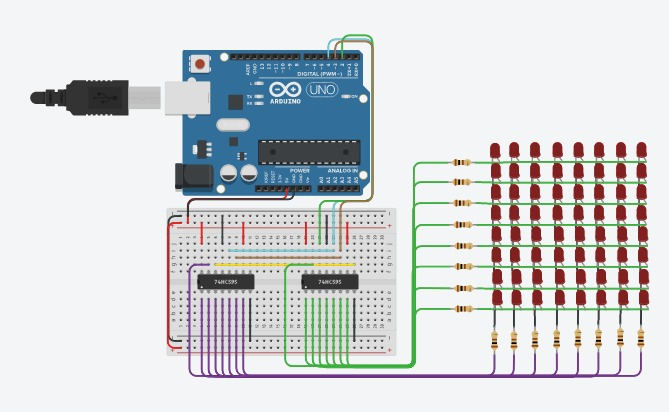
\includegraphics[width=12cm]{Dia 2.jpeg}

\vspace{0.5cm}

Para la función verificacón, que será la base para el resto de funciones, recorrimos las 8 filas de los LED y le asignamos su valor en binario, que en este caso todos bombillos deberían estar encendidos, dentro del arreglo 'ALL' utilizando la función desplazarbyte para leer los bites de cada fila y comprobar si están disponibles\\

\vspace{0.5cm}

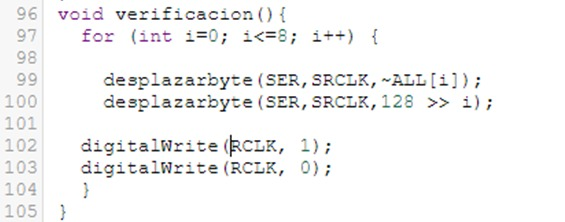
\includegraphics[width=12cm]{Veri.jpeg}

\subsection{Día 3}
\label{fig:my_label}
\section{Esquema} \label{contenido}
\begin{figure}
    \centering
    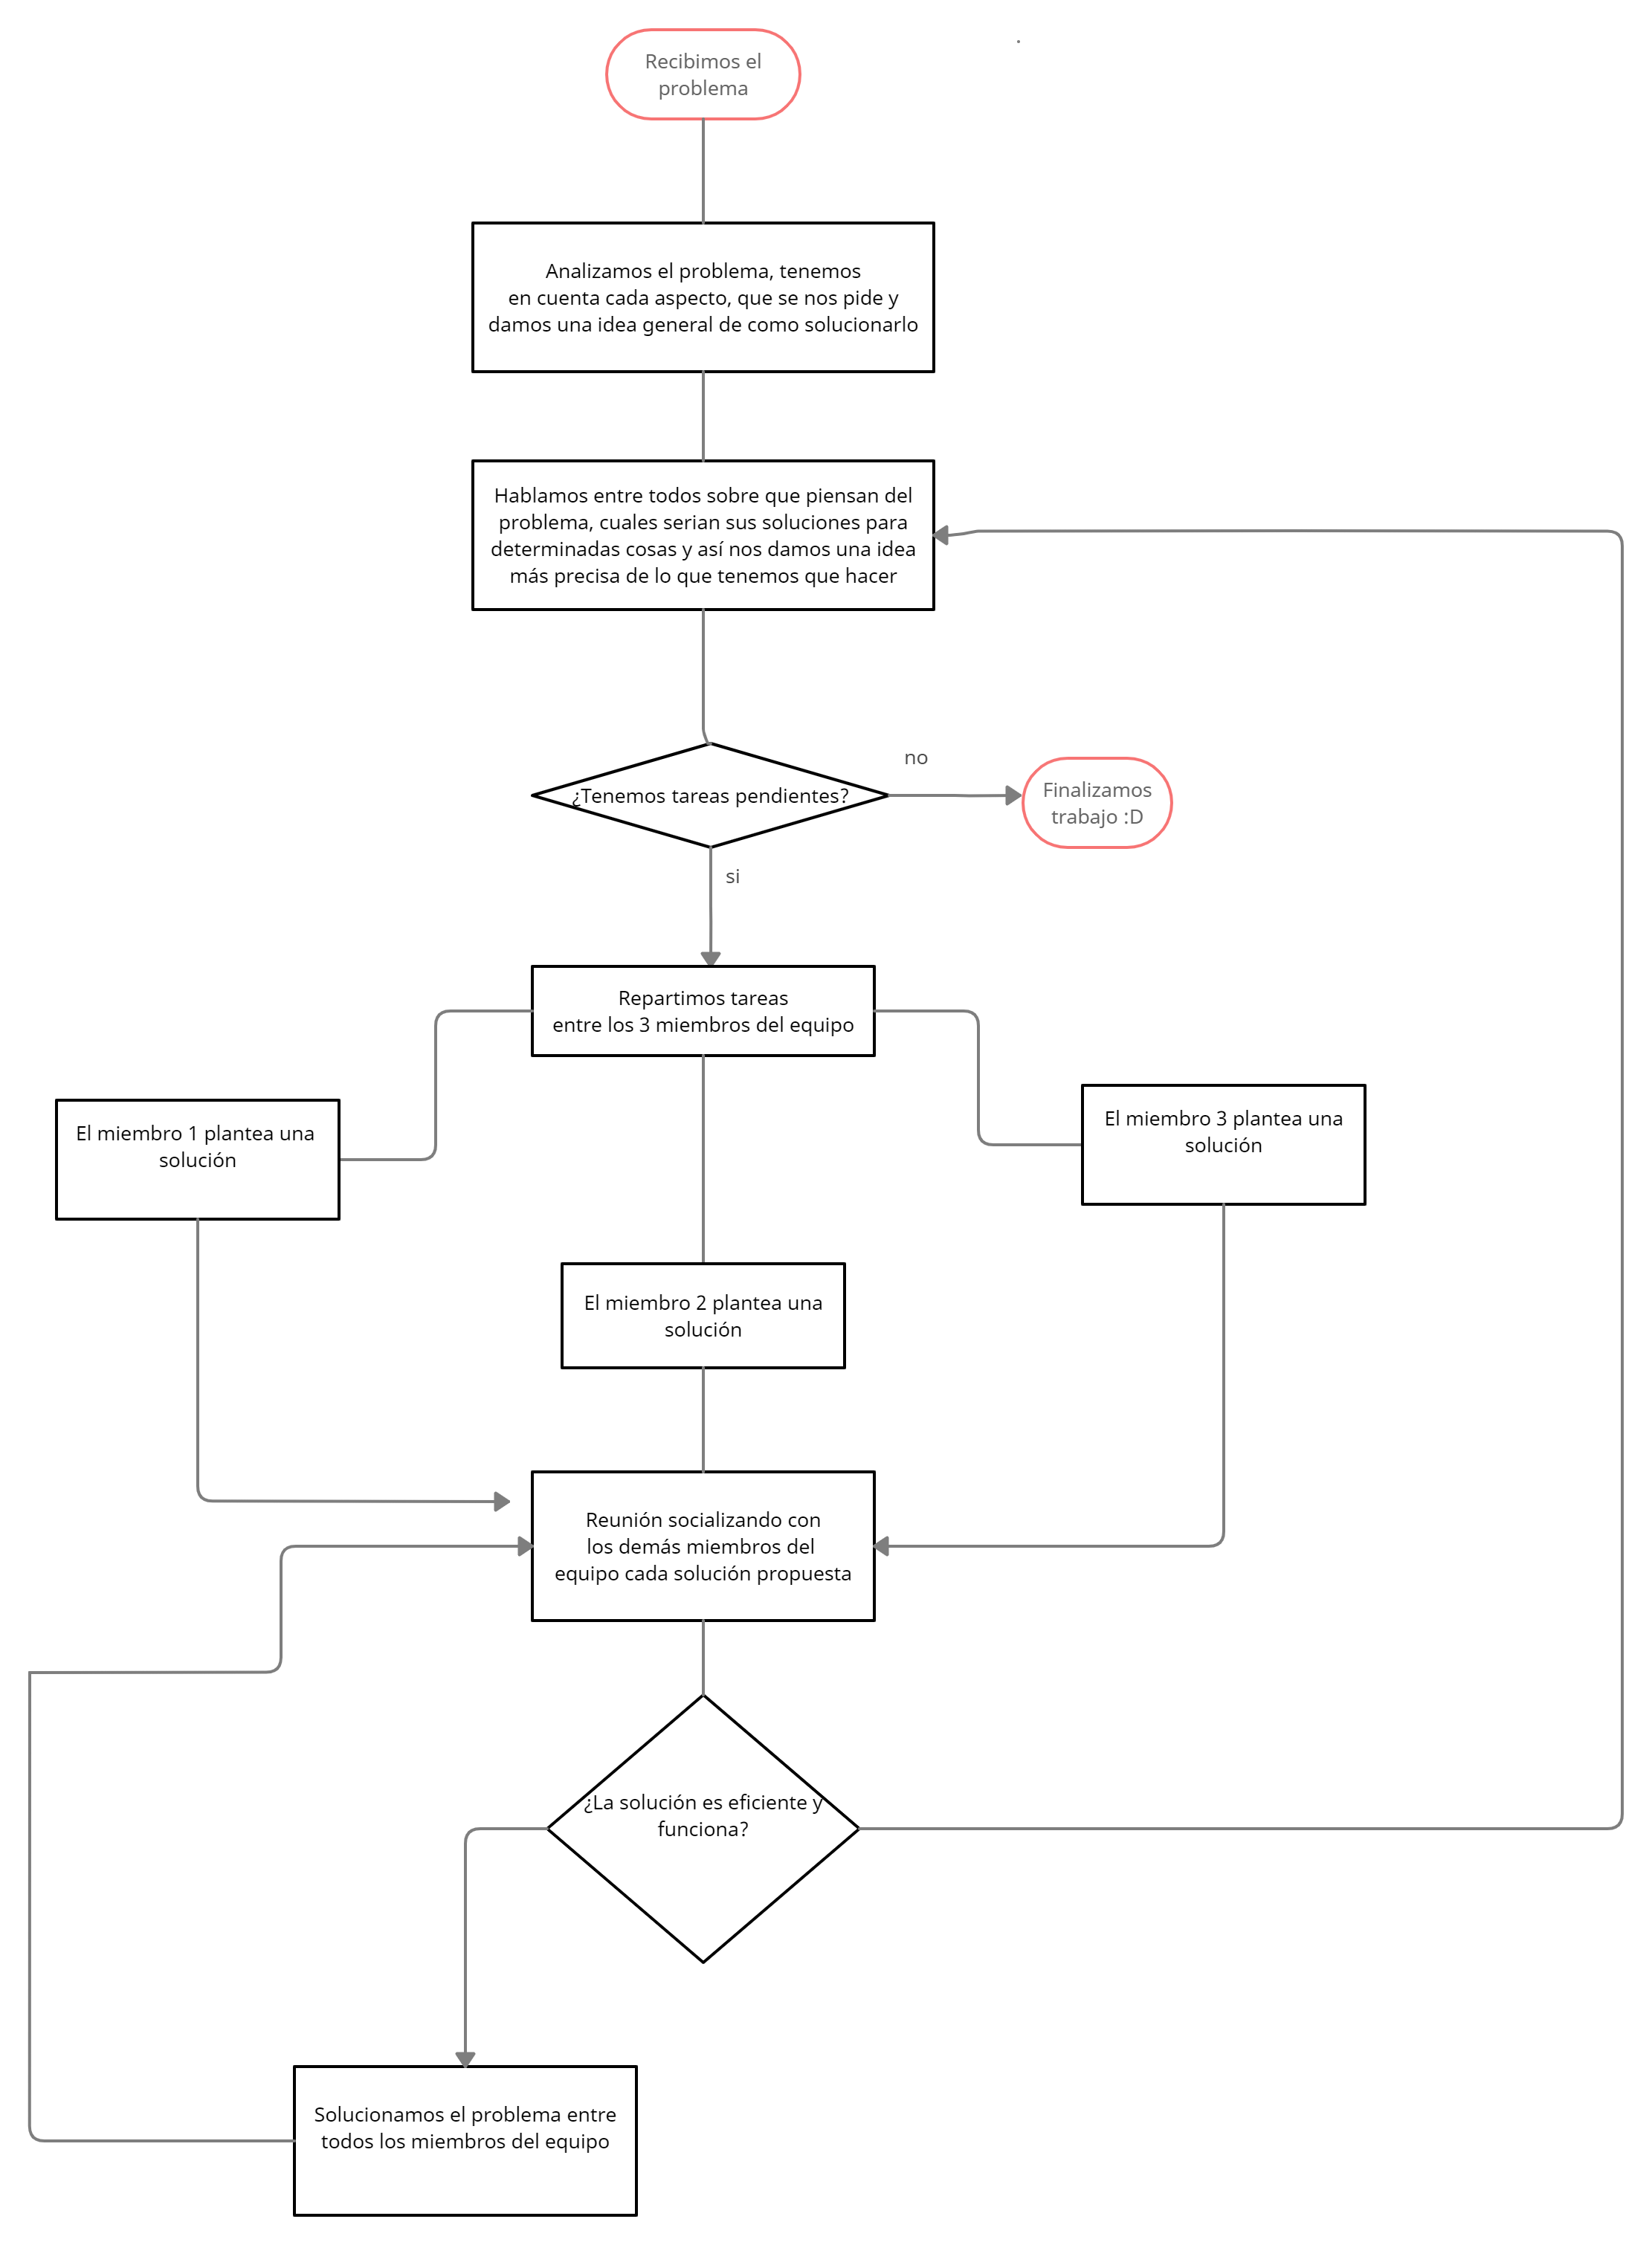
\includegraphics[width=16cm]{diagrama.png}
    \caption{diagrama}
    \label{fig:my_label}
\end{figure}
\bibliographystyle{IEEEtran}
\bibliography{references}

\end{document}